% CVPR 2026 Paper Template; see https://github.com/cvpr-org/author-kit

\documentclass[10pt,twocolumn,letterpaper]{article}

%%%%%%%%% PAPER TYPE  - PLEASE UPDATE FOR FINAL VERSION
% \usepackage{cvpr}              % To produce the CAMERA-READY version
% \usepackage[review]{cvpr}      % To produce the REVIEW version
\usepackage[pagenumbers]{cvpr} % To force page numbers, e.g. for an arXiv version

% Import additional packages in the preamble file, before hyperref
%% This file contains a number of tweaks that are typically applied to the main document.
%% They are not enabled by default, but can be enabled by uncommenting the relevant lines.

%%
%% Inline annotations; for predefined colors, refer to "dvipsnames" in the xcolor package:
%% https://tinyurl.com/overleaf-colors
%%
\newcommand{\red}[1]{{\color{red}#1}}
\newcommand{\todo}[1]{{\color{red}#1}}
\newcommand{\TODO}[1]{\textbf{\color{red}[TODO: #1]}}
%%
%% disable for camera ready / submission by uncommenting these lines  
%%
% \renewcommand{\TODO}[1]{}
% \renewcommand{\todo}[1]{#1}

\usepackage{microtype}
\usepackage{xcolor}

\renewcommand{\paragraph}[1]{\vspace{.4em}\noindent\textbf{#1}}

\setlength{\abovecaptionskip}{.4em}
\setlength{\belowcaptionskip}{.2em}

\setcounter{topnumber}{5}
\setcounter{bottomnumber}{3}
\setcounter{dbltopnumber}{5}
\setcounter{totalnumber}{8}
\renewcommand{\topfraction}{0.98}
\renewcommand{\bottomfraction}{0.6}
\renewcommand{\dbltopfraction}{0.98}
\renewcommand{\textfraction}{0.02}
\renewcommand{\floatpagefraction}{0.6}


%%
%% Allows "the use of \paper to refer to the project name"
%% with automatic management of space at the end of the word
%%
% \usepackage{xspace}
% \newcommand{\paper}{ProjectName\xspace}

%%
%% Commonly used math definitions
%%
% \DeclareMathOperator*{\argmin}{arg\,min}
% \DeclareMathOperator*{\argmax}{arg\,max}

%%
%% Tigthen underline
%%
% \usepackage{soul}
% \setuldepth{foobar}

% It is strongly recommended to use hyperref, especially for the review version.
% hyperref with option pagebackref eases the reviewers' job.
% Please disable hyperref *only* if you encounter grave issues, 
% e.g. with the file validation for the camera-ready version.
%
% If you comment hyperref and then uncomment it, you should delete *.aux before re-running LaTeX.
% (Or just hit 'q' on the first LaTeX run, let it finish, and you should be clear).
\definecolor{cvprblue}{rgb}{0.21,0.49,0.74}
\usepackage[pagebackref,breaklinks,colorlinks,allcolors=cvprblue]{hyperref}

%%%%%%%%% PAPER ID
\def\paperID{n/a}
\def\confName{CS~5788}
\def\confYear{2026}

%%%%%%%%% TITLE
\title{LaughTuned: Comparing DPO and KTO for Comedy Writing under Context Length Variation}

%%%%%%%%% AUTHORS
\author{Pranav Dhingra\\
Cornell Tech, Cornell University\\
{\tt\small pd453@cornell.edu}
}

\begin{document}
\maketitle
\begin{abstract}
We compare two preference-optimization methods, Direct Preference Optimization (DPO) and Kahneman--Tversky Optimization (KTO), as a way to align a language model to write humor about current events.  We fine-tune Mistral-7B-Instruct-v0.2 with from-scratch implementations of both losses on comedy prompts built from Guardian news articles, and vary the prompt context length: a short condition (today's headline and lede only) and a long condition that also includes a model-generated backstory summarizing recent related coverage.  This gives four trained variants.  Evaluated against the base model by an LLM cross-judge on a held-out set of 30 prompts, short-context training wins 62\% of comparisons, while long-context training wins only 47\% (worse than no fine-tuning at all).  The long-context KTO variants reach the lowest validation losses of the four runs but the cross-judge ranks them no better than base, and instrumenting the loss shows why: their mean policy-vs-reference log-probability ratio collapses to large negative values during training, indicating the policy has drifted far from the reference, while KTO's bounded loss never reflects that drift.  The practical message: under bounded surrogate losses, validation loss alone is not a reliable training signal, and longer contexts can hurt rather than help.
\end{abstract}

\section{Introduction}
\label{sec:intro}

\paragraph{Why humor, and why context length.}
Humor is a useful stress test for language-model alignment.  Unlike factual question answering, comedic writing is judged on style, surprise, and topical specificity rather than on verifiable correctness, and good outputs are diverse.  Good comedy is also rooted in context: stand-up comedians do not invent material in a vacuum, they riff on what is happening now and often connect today's events to something that already happened, producing a sort of full-circle callback.  We test whether either ingredient transfers to a fine-tuned language model by varying the prompt context length: a \emph{short} prompt that grounds the model in a current news article only, and a \emph{long} prompt that additionally injects a model-generated summary of related older coverage.  If contextual grounding matters the way it does for human comedians, longer context should produce richer comedic takes; if it doesn't, that is a finding in itself.

\paragraph{Related work.}
RLHF \cite{ouyang2022training,stiennon2020learning} showed that even noisy preference labels can steer large models.  Direct Preference Optimization (DPO) \cite{rafailov2023direct} reformulates the RLHF objective as a closed-form loss over a reference policy, eliminating the explicit reward model.  Kahneman--Tversky Optimization (KTO) \cite{ethayarajh2024kto} generalizes to binary thumbs-up/thumbs-down labels using a prospect-theoretic utility, removing the need for paired preferences.  The closest prior study on humor is \cite{zhang2024humor}, which benchmarks PPO and DPO on multimodal cartoon captioning and reports clear limitations of both; KTO is not evaluated there.  How preference optimization behaves on \emph{text-only} creative generation, and how the prompt context length interacts with the algorithm choice, has received little empirical attention.

\paragraph{Approach.}
We compare DPO and KTO on a comedy-writing task built from Guardian news articles.  We sample two candidate responses per prompt from a frozen Mistral-7B-Instruct-v0.2 \cite{jiang2023mistral}, score each on a three-axis humor rubric using an external judge (Claude Sonnet 4.6), and derive paired (for DPO) and binary (for KTO) datasets from the same scored pool.  Four LoRA-adapted variants \cite{hu2021lora,dettmers2023qlora} are then trained: DPO and KTO under both \emph{short} (headline + lede only) and \emph{long} (plus a model-generated backstory from related older articles) prompts.  Our DPO and KTO losses are implemented from scratch in PyTorch (no Transformer Reinforcement Learning (TRL) or other preference-optimization library), which lets us directly instrument internal quantities such as policy-vs-reference log-probability ratios that high-level training APIs hide.  Evaluation uses an LLM cross-judge on 30 held-out prompts (rank-3 forced choice) plus a parallel blinded ranking by the author.

\paragraph{Contributions.}
(i) Reproducible from-scratch DPO and KTO implementations that match the published formulations and expose internal training metrics for diagnostic plotting.  (ii) Empirical evidence that prompt context length matters as much as the algorithm choice: short-context training improves both algorithms over the base model while long-context training degrades them, under identical hyperparameters.  (iii) A concrete failure mode for KTO: its validation loss falls monotonically while the policy drifts far from the reference, but the bounded loss never registers the drift, so val-loss alone is unsafe as a stopping criterion.  (iv) An algorithm-context interaction: DPO beats KTO head-to-head on short contexts, KTO beats DPO on long contexts.

\section{Method}
\label{sec:method}

\begin{figure*}[t]
\centering
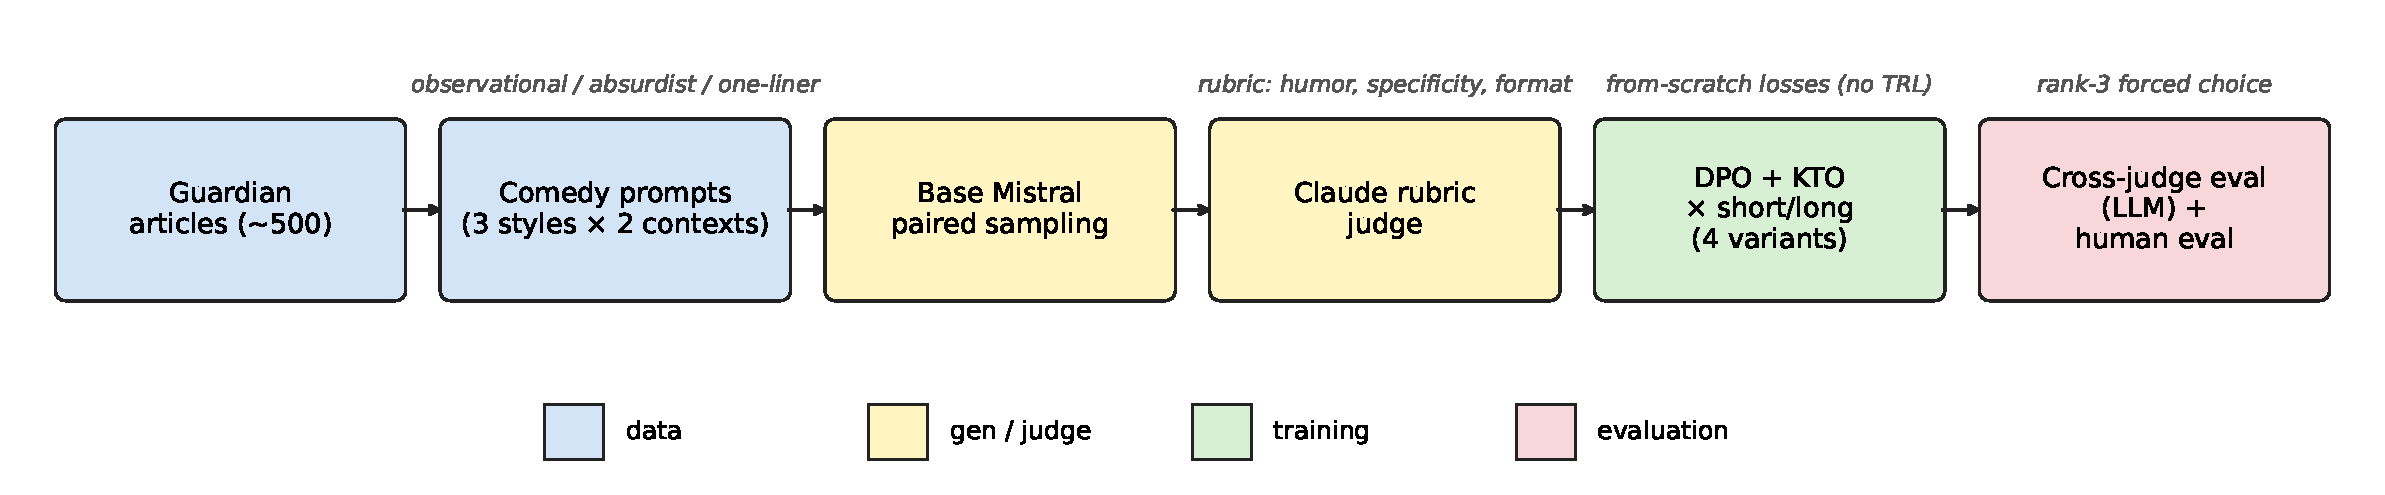
\includegraphics[width=0.98\linewidth]{figures/pipeline.pdf}
\caption{End-to-end pipeline: Guardian articles to LoRA-tuned variants to cross-judge + human evaluation.}
\label{fig:pipeline}
\end{figure*}

\subsection{Data construction}
We fetch 502 articles from the Guardian Open Platform API spanning eight sections (politics, business, technology, sport, culture, science, environment, world) and build one comedy prompt per article.  Each prompt is randomly assigned one of three styles (observational, absurdist, or one-liner), with the style label only affecting the role and task instructions; the rest of the template is identical across prompts.

\paragraph{Short vs.\ long context.}
Every prompt has two variants that differ only in their context body.  The \textbf{short} variant contains the article's headline and the first $\sim$400 tokens of the body.  The \textbf{long} variant prepends a model-generated $\sim$150-word historical backstory: we run a topic query extracted from the headline through the Guardian search API (1--18 month lookback ending two weeks before publication), retrieve the three most relevant older articles, and have Claude Sonnet 4.6 summarize them.  The role/task/output-format wording is identical across both variants, so the only experimental factor is the context body.  Figure~\ref{fig:prompt} shows the exact template with the long-only insert highlighted.

\begin{figure}[t]
\centering
\small
\setlength{\fboxsep}{4pt}
\colorbox{gray!8}{\parbox{0.92\linewidth}{\small
\texttt{<role>}You are a sharp observational comedian.\texttt{</role>}\\[2pt]
\texttt{<context>}\\
\colorbox{cyan!20}{\parbox{0.84\linewidth}{\textbf{\textit{[long only]}} \texttt{<background>}~A 150-word factual recap synthesized by Claude Sonnet 4.6 from up to three older Guardian articles retrieved via topic-query search.~\texttt{</background>}}}\\
\texttt{<latest>}~Headline + first $\sim$400 tokens of today's article body.~\texttt{</latest>}\\
\texttt{</context>}\\[2pt]
\texttt{<task>}Write a short, specific comedic take (2--3 sentences). Reference real details from the context.\texttt{</task>}\\[2pt]
\texttt{<output\_format>}Respond with only the joke. No preamble or quotation marks.\texttt{</output\_format>}
}}
\caption{Prompt template (observational style).  \colorbox{cyan!20}{Shaded region} appears only in the long variant; the rest is identical across short/long and across styles.}
\label{fig:prompt}
\end{figure}

\paragraph{From articles to preferences.}
We split 30 prompts off as the held-out evaluation set and use the remaining 472 for training/validation (10\% val).  For each training prompt we sample two candidate responses from the frozen base model at $T{=}0.9$, $p{=}0.95$ and score each with Claude Sonnet 4.6 against a fixed three-axis humor rubric: \textbf{context engagement}, \textbf{comedic technique}, and \textbf{surprise} (1--5 each, taken from a single judge call).  Let $c$ be the mean of the three sub-scores.  Two datasets are then derived from the \emph{same} scored pool:
\begin{itemize}\itemsep1pt\parsep0pt
\item \textbf{Paired preferences} (for DPO): per prompt, the higher-$c$ response is the chosen, the other is the rejected.
\item \textbf{Binary labels} (for KTO): responses with $c \geq 3.0$ are marked desirable, responses with $c \leq 2.5$ are marked undesirable, intermediate $c$ are dropped.
\end{itemize}
This co-derived sampling pool isolates the loss-function comparison from a data-pipeline confound that would arise if DPO and KTO were trained on independently-collected datasets.

\subsection{From-scratch DPO and KTO}
Implementing both losses from scratch lets us instrument internal quantities (particularly the policy-vs-reference log-probability ratio) that high-level training APIs hide, which is what makes the policy-drift diagnostic in Section~\ref{sec:experiments} possible.

\paragraph{DPO loss.} For paired data $(y_w, y_l)$ with implicit reward $r_\theta(x,y) = \log \pi_\theta(y|x) - \log \pi_\text{ref}(y|x)$,
\begin{equation}
\mathcal{L}_\text{DPO} = -\mathbb{E}\left[\log \sigma\!\left(\beta (r_\theta(x,y_w) - r_\theta(x,y_l))\right)\right].
\end{equation}

\paragraph{KTO loss.} For binary-labeled data with per-batch reference $z_\text{ref} = \operatorname{stop\_grad}(\mathbb{E}[r_\theta])$,
\begin{align}
v(x,y) &= \begin{cases} \sigma(\beta(r_\theta - z_\text{ref})) & \text{if } y \text{ desirable} \\ \sigma(\beta(z_\text{ref} - r_\theta)) & \text{if } y \text{ undesirable}\end{cases} \\[2pt]
\mathcal{L}_\text{KTO} &= \mathbb{E}\big[\lambda_y \cdot (1 - v(x,y))\big],
\end{align}
where $\lambda_\text{desirable}$ and $\lambda_\text{undesirable}$ are inverse class frequencies that rebalance the batch.  $\mathcal{L}_\text{KTO}$ is bounded in $[0, \max(\lambda_d, \lambda_u))$ regardless of how far $r_\theta$ drifts from $z_\text{ref}$; this bounded-loss property becomes important in Section~\ref{sec:ktodrift}.

\subsection{Training configuration}
Table~\ref{tab:hp} lists training hyperparameters, shared across all four variants on a single NVIDIA A100 GPU on Google Colab; only loss type and context length vary.

\begin{table}[t]
\centering
\small
\begin{tabular}{ll}
\toprule
Hyperparameter & Value \\
\midrule
Base model & Mistral-7B-Instruct-v0.2 \\
Quantization & 4-bit NF4 (QLoRA) \\
LoRA rank / $\alpha$ / dropout & 16 / 32 / 0.05 \\
LoRA target modules & q,k,v,o projections \\
Max sequence length & 1024 tokens \\
Optimizer & AdamW (paged) \\
Learning rate & $1{\times}10^{-5}$ \\
LR schedule & cosine, 10\% warmup \\
Effective batch size & 32 ($16 \times 2$ accum) \\
Max grad norm & 1.0 \\
$\beta$ (DPO and KTO) & 0.1 \\
Epochs & 10 (with early stopping) \\
Eval / save interval (steps) & 10 / 20 \\
Early-stopping patience & 5 evals \\
\bottomrule
\end{tabular}
\caption{Training hyperparameters.}
\label{tab:hp}
\end{table}

\subsection{Evaluation protocol}
For each trained variant we generate one response per held-out prompt using the \emph{best-validation-loss adapter checkpoint} for that variant (the same adapter the training loop reloads on exit after early stopping), with the base Mistral generation hyperparameters ($T{=}0.9$, $p{=}0.95$, $\text{max\_new\_tokens}{=}200$).  We evaluate every variant on the 30-prompt held-out split with two complementary signals.  The primary signal is an \textbf{LLM cross-judge}: for each prompt and each comparison (base vs DPO, base vs KTO, DPO vs KTO), the judge ranks all three generations under randomized letter labels, and we read pairwise win rates from the rank-3 ordering.  As a \textbf{secondary, human-grounded} signal, the author performed the same blinded rank-3 ranking on 30 sampled triplets (15 short + 15 long, interleaved with no context-length label); we report pairwise agreement between the two judges as a sanity check on the cross-judge.  As a fluency check we also report \textbf{perplexity} of the generated jokes under the frozen base model: it catches collapsed or off-distribution generations even when the cross-judge cannot articulate why.

\section{Experiments}
\label{sec:experiments}

\begin{figure*}[!t]
\centering
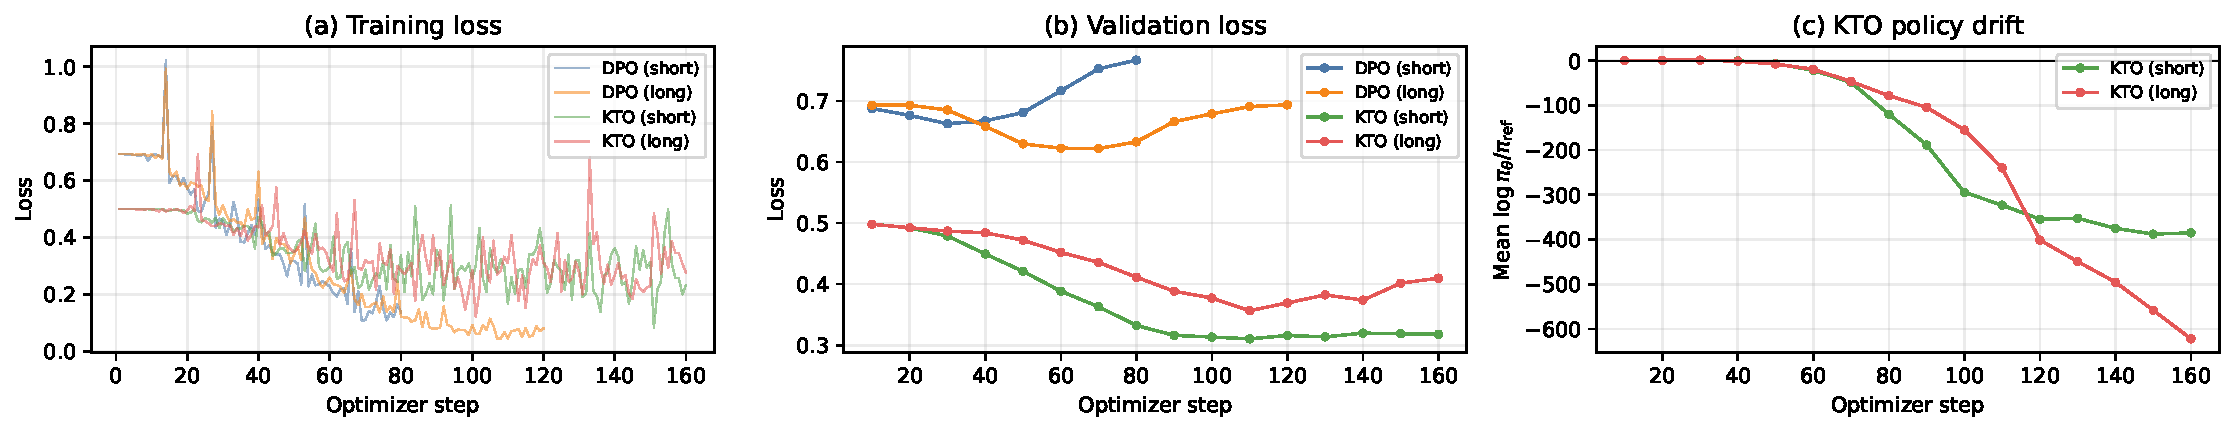
\includegraphics[width=\linewidth]{figures/training_curves.pdf}
\caption{Training diagnostics: (a) training loss, (b) validation loss, (c) KTO validation log-ratio $\mathbb{E}[\log \pi_\theta / \pi_\text{ref}]$.  KTO's log-ratio collapse (panel c) is discussed in \S\ref{sec:ktodrift}.}
\label{fig:training}
\end{figure*}

\begin{figure*}[!t]
\centering
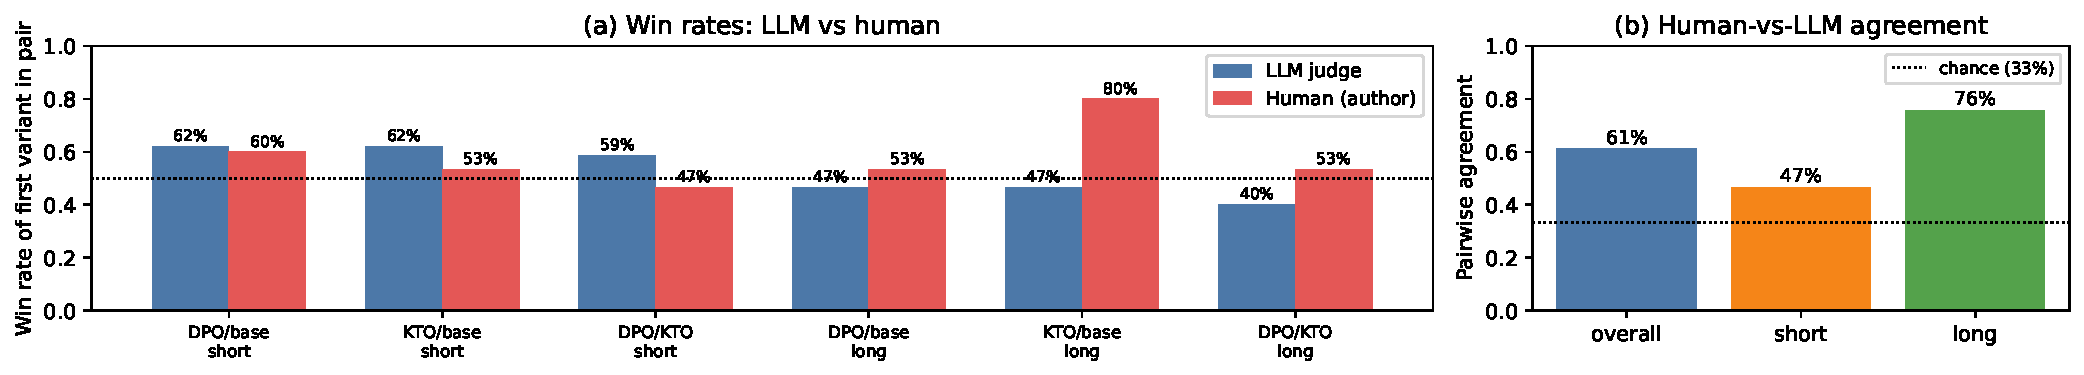
\includegraphics[width=\linewidth]{figures/agreement_matrix.pdf}
\caption{LLM vs human win rates per comparison (left) and pairwise agreement breakdown (right).}
\label{fig:agree}
\end{figure*}

\subsection{Data and splits}
The 502 prompts are split 30 / 472, with 30 held out for evaluation and the remaining 472 split 90/10 into train and val.  Class balance on the KTO binary task is uneven (37\% desirable, 59\% undesirable in the short condition), which makes KTO's inverse-frequency weighting load-bearing rather than cosmetic.

\subsection{Training dynamics}
Best-val-loss checkpoint selection (Figure~\ref{fig:training}a,b) picks step~30 for DPO short, 70 for DPO long, and 110 for both KTO variants.  DPO overfits visibly in the second half (train collapses, val rises); KTO long bottoms then degrades.

\subsection{Cross-judge results}
The dominant pattern in the cross-judge rankings is a context-length effect: short-context fine-tuning improves both algorithms over the base model (DPO 62\%, KTO 62\%), while long-context fine-tuning \emph{degrades} both below base (DPO 47\%, KTO 47\%).  Head-to-head, DPO beats KTO on short (59--41) while KTO beats DPO on long (60--40), suggesting algorithm choice should be made jointly with context length rather than independently.  Table~\ref{tab:quant} consolidates these numbers alongside the validation losses and reveals a disagreement: KTO achieves lower val loss than DPO in both context conditions (0.310 vs 0.663 short; 0.357 vs 0.622 long), yet the cross-judge ranks the two in the \emph{opposite} order on the short condition.  The mechanism is in \S\ref{sec:ktodrift}.

\begin{table}[!htb]
\centering
\small
\setlength{\tabcolsep}{6pt}
\begin{tabular}{lccc}
\toprule
Variant & Val loss $\downarrow$ & WR vs base $\uparrow$ & Perp.\ $\downarrow$ \\
\midrule
Base short              & ---    & ---  & 3.25 \\
DPO short    & 0.663  & 0.62 & 2.68 \\
KTO short    & 0.310  & 0.62 & 2.97 \\
\midrule
Base long               & ---    & ---  & 2.88 \\
DPO long    & 0.622  & 0.47 & 3.02 \\
KTO long    & 0.357  & 0.47 & 2.95 \\
\bottomrule
\end{tabular}
\caption{Quantitative results.  Win rate is against base on the matching context; perplexity is under the frozen base model.}
\label{tab:quant}
\end{table}

\subsection{KTO's validation loss masks policy drift}
\label{sec:ktodrift}
KTO's loss has an upper bound: once the policy is confidently wrong enough, the loss saturates near its cap and stops giving the optimizer useful gradient, but nothing in the loss prevents the policy from drifting further from the reference.  Figure~\ref{fig:training}(c) shows this happening: validation loss falls monotonically while the mean validation log-ratio $r_\theta = \log\pi_\theta - \log\pi_\text{ref}$ crashes to $\sim-400$ (KTO short) and below $-600$ (KTO long).  At those values the trained policy is assigning the average eval response a probability $\sim e^{-400}$ times the reference, which is effectively a different model and is consistent with KTO long's 47\% cross-judge win rate against base.  DPO does not collapse this way because its loss is unbounded; if the margin goes the wrong way, $-\log\sigma$ blows up and the optimizer is forced to fight drift.

Pal et al.\ \cite{pal2024smaug} reported a related issue in DPO where the chosen-response probability can drop below the reference, and patched it with an added regularizer (DPO-Positive).  We see KTO's analog as not needing a regularizer at all: the policy-vs-reference log-ratio is already directly observable during training, and gating on it rather than on validation loss is enough to catch this failure mode.

\paragraph{Human validation.}
\label{sec:humanval}
Figure~\ref{fig:agree} compares the two judges.  Pairwise agreement (protocol in \S\ref{sec:method}) is 61\% overall (Cohen's $\kappa = 0.34$ on the top pick), asymmetric by context: long 76\%, short 47\% (short-context distinctions are subtle).  The biggest disagreement is KTO long vs base, where humans pick KTO long 80\% of the time but the LLM only 47\%.

\paragraph{Qualitative.}
On a one-liner prompt about British Airways' £1.7bn fuel hit and the Iran war:

\noindent\textbf{Base.}  ``Why don't British Airways fly Boeing 747s anymore? Because those fuel bills are so high, they'd need to charge a premium BA fare just to fill up the jumbo jets.''  (Generic; the article isn't really doing any work.)

\noindent\textbf{DPO short.}  ``Why did British Airways increase their prices like a hot air balloon? To recover the €2bn fuel bill from the Iran-Iraq price war.''  (Pulls in the actual numbers and the geopolitical hook.)

\noindent\textbf{KTO short.}  ``Why did British Airways hike up their premium fares? To cover the £1.7bn unexpected fuel bill they incurred after buying tickets to Iran's war of words and lost their fuel hedging bet?''  (Article-specific and includes a finance term, but punchline meanders.)

On the same prompt in long context, the base model emits the literal tag \verb|<alternate_jokes>| inside its response, a representative prompt-template leakage discussed in the limitations.

\section{Conclusion}
\label{sec:conclusion}

\enlargethispage{4\baselineskip}
Under identical hyperparameters, short-context fine-tuning improves both DPO and KTO over the base model (62\% cross-judge win rate) while long-context fine-tuning \emph{degrades} both (47\%); the prompt-context length matters as much as the algorithm choice.  The two algorithms also interact with context length: DPO wins short head-to-head (59--41), KTO wins long (60--40).  Most striking, KTO's validation loss is misleading: both KTO runs reach lower val loss than DPO, yet the cross-judge ranks them no better; their mean policy-vs-reference log-ratio collapses to ${\sim}{-400}$ (short) and ${\sim}{-600}$ (long) at the best-val checkpoint while KTO's bounded loss never registers the drift.  \textbf{Take-away}: with a bounded preference-optimization surrogate like KTO, validation loss alone is not a safe stopping criterion; the policy-vs-reference log-ratio is cheap to monitor and is the signal that actually catches catastrophic drift.

\paragraph{Limitations.}
(i) $\sim$5--10\% of generations from every variant emit literal XML tags from the prompt template; Mistral-Instruct was tuned on \texttt{[INST]} delimiters and our template is slightly out-of-distribution, so this affects all variants approximately equally.
(ii) 18.7\% of training articles and 20\% of eval prompts had no usable backstory (Guardian search in-window returned nothing), partially contaminating the long-context arm.
(iii) $\sim$47\% of eval prompts touch tragic topics that simply don't make good comedy; not filtered.
(iv) the human eval was conducted by the author alone, so there is no external or majority agreement of the ranking.

{
    \small
    \bibliographystyle{ieeenat_fullname}
    \bibliography{main}
}
\appendix
\section{AI Usage}
\label{sec:aiuse}

The author used \textbf{Claude Code} (Anthropic) as a pair-programming assistant, primarily helping set up pipelines for dataset generation, evaluation, and figure generation. It was also used for housekeeping tasks like updating the repo README, adding docstrings to functions and modules, and formatting the report in LaTeX. The core parts of training and evaluation were written by the author (e.g. DPO/KTO loss functions, training loop, LLM prompt-template, eval rubric, etc.). All code was reviewed by the author before being committed. All scientific decisions (algorithm choice, evaluation design, hyperparameter selection, claim formulation, limitations analysis) were made by the author.



\end{document}
